\documentclass[11pt,a4paper]{article}
\usepackage[T1]{fontenc}
\usepackage[margin=2.3cm]{geometry}
\usepackage{amsmath,amssymb}
\usepackage{graphicx}
\usepackage[dvipsnames]{xcolor}
\usepackage{enumitem}
\usepackage[colorlinks=true,linkcolor=blue,urlcolor=blue]{hyperref}
\setlength{\parskip}{0.6em}
\setlength{\parindent}{0pt}
\begin{document}

\begin{center}{\LARGE\bfseries openneuralode}\\[0.4em]{\large Learn how things change from data: neural ODEs in three sessions.}\\[0.2em]\small PAN IIT OSS explainer \textbullet{} higher secondary to advanced undergraduate (levels 4-6)\end{center}

\section*{Why this exists}
Many systems, from a spring to a chemical reaction, change according to a rule dx/dt = f(x). This explainer shows how the rule can be pictured, solved and then learned from noisy data by a small neural network, using only arrows, a solver and the chain rule, so you can build it yourself.

\section*{The end goal}
Learn dynamics from data with neural ODEs. The end goal is learning dynamics from data with neural ODEs, as used in science and engineering when the equations are unknown or too costly to simulate. The same ideas let a model be trained through a physical solver instead of treating the data as a pile of unrelated points.

\section*{How the three sessions build up}
\begin{enumerate}[nosep]
\item \textbf{Session 1: A rule for change: dx/dt = f(x)} (Level 1, conceptual interactive model, 60 min).
\item \textbf{Session 2: Solvers, least squares and a first neural network} (Level 2, mathematical engineering model, 75 min).
\item \textbf{Session 3: A Neural ODE trained through the solver} (Level 3, simulation and validation, 90 min).
\end{enumerate}

\section{Session 1: A rule for change: dx/dt = f(x)}

\subsection*{A. Real-world problem}
A mass hangs on a spring and wobbles to a stop. You could try to write the whole path as a formula, or you could ask a smaller question that is true at every instant: if the mass is HERE and moving THIS fast, how is it changing right now? The answer is a rule dx/dt = f(x). Once you have the rule, a computer can predict the path from any start. A neural network can learn the rule f from recorded positions, even when you do not know the physics. How do we picture such a rule, and how do we get it from data?

\subsection*{B. Concept and theory}
The state of the system is a list of numbers; for the spring it is the pair (x, v): position and velocity. The rule f gives, for every state, an arrow showing how the state is changing: its first number is dx/dt and its second is dv/dt. Following the arrows means: start somewhere, move a short time dt along the arrow, look at the new arrow, repeat. The paths you get never cross, because the rule depends only on where you are. For the spring with friction the rule is dx/dt = v and dv/dt = -k x - c v: the spring pulls back in proportion to the stretch and friction slows the motion. With k = 4 and c = 0.4 the path is a spiral: the mass swings back and forth with angular frequency sqrt(k - c\textasciicircum{}2/4), about 1.99 rad/s, and the size of the swing shrinks like exp(-c t / 2). To read the rule from observations, take two neighbouring snapshots and divide the change by the time between them.

\begin{itemize}[nosep]
\item x: position of the mass from its rest point (m)
\item v: velocity of the mass (m/s)
\item k: spring stiffness divided by mass (1/s\textasciicircum{}2)
\item c: friction divided by mass (1/s)
\item f(x, v): the arrow: (dx/dt, dv/dt) at a state (m/s and m/s\textasciicircum{}2)
\item dt: time between recorded snapshots or between solver steps (s)
\end{itemize}

\begin{equation*}
\frac{dx}{dt}=v,\qquad \frac{dv}{dt}=-k\,x-c\,v
\end{equation*}

\begin{equation*}
\mathbf s_{\text{next}}=\mathbf s+\Delta t\,f(\mathbf s)\quad\text{(one step along the arrow)}
\end{equation*}

\begin{equation*}
f_{\text{estimated}}\approx\frac{\mathbf s_{i+1}-\mathbf s_i}{\Delta t}
\end{equation*}

\begin{equation*}
x(t)=e^{-ct/2}\Big(\cos\omega_d t+\frac{c}{2\omega_d}\sin\omega_d t\Big),\qquad \omega_d=\sqrt{k-c^2/4}
\end{equation*}

\begin{center}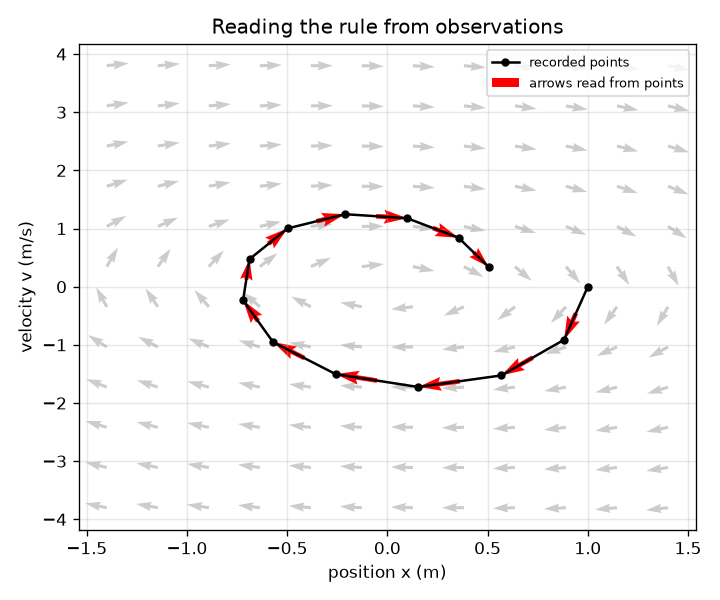
\includegraphics[width=0.85\linewidth]{figures/s01_arrows_from_data.png}\\\small Recorded points (black) and the arrows read from them (red) lie along the true arrows (grey).\end{center}

\subsection*{E. Worked example}
For k = 4 and c = 0.4, find the arrow at the state (x, v) = (1 m, 0) and at (0, 2 m/s), and take one step of 0.1 s along the first arrow.
\begin{enumerate}[nosep]
\item At (1, 0): dx/dt = v = 0 and dv/dt = -4 * 1 - 0.4 * 0 = -4 m/s\textasciicircum{}2. The arrow is (0, -4): the mass is momentarily at rest and starts to speed up towards the rest point.
\item At (0, 2): dx/dt = 2 m/s and dv/dt = -4 * 0 - 0.4 * 2 = -0.8 m/s\textasciicircum{}2. The arrow is (2, -0.8): the mass moves forward and friction slows it slightly.
\item One step of 0.1 s from (1, 0): new state = (1, 0) + 0.1 * (0, -4) = (1.0, -0.4).
\item Check by thought: after 0.1 s the mass has barely moved (still about 1 m) and has picked up a velocity of about -0.4 m/s. That is reasonable.
\end{enumerate}
\textbf{Answer.} The arrow at (1, 0) is (0, -4) and the arrow at (0, 2) is (2, -0.8). One step of 0.1 s from (1, 0) lands at (1.0, -0.4).

\subsection*{F. Questions}
\begin{enumerate}[nosep]
\item \textbf{Conceptual.} At the state (1 m, 0) the arrow is (0, -4). Why is the first number zero even though the mass is about to move?
\item \textbf{Numerical.} For k = 4 and c = 0.4, find the arrow at (0, 2 m/s) and the state after one step of 0.1 s along it. Give units and check that the answer is reasonable.
\item \textbf{Graph and simulation interpretation.} In the phase view, why does the path spiral inwards when friction c is above 0 and form a closed loop when c = 0? Where would the path end?
\item \textbf{Design and optimisation challenge.} Design: you record the mass with a sensor that gives a snapshot every dt seconds, and you want the arrows read from neighbouring snapshots to be within 1 percent of the true rule. Is dt = 0.25 s good enough? Is 0.1 s?
\end{enumerate}

\section{Session 2: Solvers, least squares and a first neural network}

\subsection*{A. Real-world problem}
A noisy sensor watches the mass on a spring. We want a rule that predicts where the mass will be 3 seconds from now. Two things decide whether this works: how we integrate the rule (a crude solver adds its own error) and how we get the rule from noisy data (a fit can be hurt by noise, and extra data only helps up to a point). How accurate are the solvers, how well can a simple fit and a small network recover the rule, and how much data and how little noise do we need?

\subsection*{B. Concept and theory}
A solver replaces the exact path by steps of size h. Euler follows the arrow once per step; RK4 samples the arrow four times (start, two midpoints, end) and blends them with weights 1, 2, 2, 1 over 6. The error at a fixed time T behaves like C h\textasciicircum{}p; taking logarithms gives log(error) = log C + p log h, a straight line of slope p: the order. Euler has p = 1 and RK4 has p = 4, so halving h divides the error by about 2 for Euler and by about 16 for RK4. To learn the rule from data, first estimate derivatives at each sample from its two neighbours, (x\_\{i+1\} - x\_\{i-1\}) / (2 dt) (a central difference). If we believe the rule is linear, f(x) = A x, the best A minimises the sum of squared differences between the estimated derivatives and A x: linear least squares. A neural network f(x) = W2 tanh(W1 x + b1) + b2 can represent rules that are not linear. With 16 hidden units it has 82 numbers, found by gradient descent on the mean squared difference between its output and the estimated derivatives (the one-step loss). Gradients are computed by hand with the chain rule (backpropagation) and the numbers are updated with Adam, which scales each step by a running average of recent gradients. Noise in the data is multiplied by 1/dt when we form derivatives, and noise in the inputs biases a least-squares fit, so more data helps only until this floor is reached.

\begin{itemize}[nosep]
\item h: solver step size (s)
\item p: order of accuracy (slope on log-log axes) (no unit)
\item A: 2x2 matrix of the linear rule f(x) = A x (1/s)
\item sigma: size of the sensor noise on positions and velocities (m and m/s)
\item K: number of recorded runs (each 20 samples) (no unit)
\item W1, b1, W2, b2: network weights: 16x2, 16, 2x16 and 2 numbers (no unit)
\end{itemize}

\begin{equation*}
x_{n+1}=x_n+h\,f(x_n)\quad\text{(Euler)}
\end{equation*}

\begin{equation*}
x_{n+1}=x_n+\frac h6\,(k_1+2k_2+2k_3+k_4),\; k_1=f(x_n),\; k_2=f(x_n+\tfrac h2k_1),\; k_3=f(x_n+\tfrac h2k_2),\; k_4=f(x_n+hk_3)
\end{equation*}

\begin{equation*}
\text{error}(h)\approx C\,h^{p}\;\Rightarrow\;\log(\text{error})=\log C+p\,\log h
\end{equation*}

\begin{equation*}
\hat A=\arg\min_A\sum_i\|\dot x_i-A x_i\|^2,\qquad \dot x_i\approx\frac{x_{i+1}-x_{i-1}}{2\,\Delta t}
\end{equation*}

\begin{equation*}
f_\theta(x)=W_2\tanh(W_1x+b_1)+b_2,\qquad L=\operatorname{mean}\|f_\theta(x_i)-\dot x_i\|^2
\end{equation*}

\begin{center}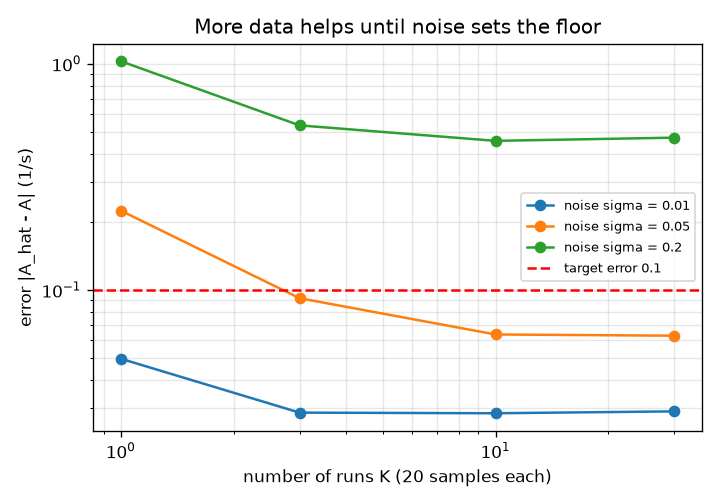
\includegraphics[width=0.85\linewidth]{figures/s02_design_table.png}\\\small Least-squares fit error against the number of runs for three noise levels; the red line is the target error 0.1.\end{center}

\subsection*{E. Worked example}
From the state (1 m, 0) with k = 4 and c = 0.4, take one step of h = 0.1 s with Euler and with RK4, and compare with the exact state.
\begin{enumerate}[nosep]
\item Euler: the arrow at (1, 0) is (0, -4), so the new state is (1, 0) + 0.1 * (0, -4) = (1.0, -0.4).
\item RK4 stage 1: k1 = (0, -4). Stage 2 at (1, 0) + 0.05 * k1 = (1, -0.2): k2 = (-0.2, -3.92). Stage 3 at (1, 0) + 0.05 * k2 = (0.99, -0.196): k3 = (-0.196, -3.8816).
\item RK4 stage 4 at (1, 0) + 0.1 * k3 = (0.9804, -0.38816): k4 = (-0.38816, -3.766336).
\item Blend: (0.1 / 6) * (k1 + 2 k2 + 2 k3 + k4) = (0.1 / 6) * (-1.18016, -23.369536) = (-0.01967, -0.38949), so the new state is (0.98033, -0.38949).
\item The exact state at t = 0.1 s is (0.9803, -0.3895). Euler is off by about 0.022 in state distance; RK4 is within 1e-5.
\end{enumerate}
\textbf{Answer.} Euler gives (1.0, -0.4), RK4 gives (0.9803, -0.3895) (equal to the exact state to 1e-5). Euler's error for this one step is about 0.022.

\subsection*{F. Questions}
\begin{enumerate}[nosep]
\item \textbf{Conceptual.} With noise 0.2 the fit error stays above 0.3 even with 30 runs, while with noise 0.01 a handful of runs is enough. Why does more data not fix the noisy case?
\item \textbf{Numerical.} The Euler error at 2 s is 0.575 for h = 0.1. Predict the error for h = 0.025 using the order p = 1, then compare with the measured value 0.128. What would an order-4 method predict from its error 4.3e-5 at h = 0.1?
\item \textbf{Graph and simulation interpretation.} In the error graph, how do you read the order of a method, and what would a slope of 2 mean? What happens to RK4 if h becomes extremely small?
\item \textbf{Design and optimisation challenge.} Design: the sensor noise can be 0.01, 0.05 or 0.2 and you can record K = 1, 3, 10 or 30 runs of 20 samples. You need a fit error (\textbar{}A\_hat - A\textbar{}) below 0.1. Which combinations work, and which sensor and how many runs would you choose?
\end{enumerate}

\section{Session 3: A Neural ODE trained through the solver}

\subsection*{A. Real-world problem}
In Session 2 the network was trained on single steps. When the sensor is noisy, the noise leaks into the learned rule, and small mistakes in the rule pile up when we predict many steps ahead. A Neural ODE changes what we train: the network is the right-hand side of an ODE, the ODE is solved with RK4, and the loss is measured on the solver's output several steps later. Does that give better long predictions? How do we know the learned flow is right? And where does the whole idea break?

\subsection*{B. Concept and theory}
The model is dx/dt = f\_theta(x) with f\_theta(x) = W2 tanh(W1 x + b1) + b2 (width 12: 62 numbers). Starting from every observed state we run m RK4 steps of size 0.1 s and compare each step with the next observation; the loss is the mean squared difference. m = 1 is the one-step loss through the solver, m = 8 the rollout loss. To minimise it we need the gradient of the loss with respect to the 62 numbers. We compute it by hand-coded backpropagation through the RK4 steps (discretise then optimise): the sensitivity of the loss to the state after a step is pushed back through the four stages in reverse order, each stage using the network's vector-Jacobian product. This gives the exact gradient of the discrete loss, which we check against finite differences in the checkpoint. The adjoint method, described here only as a concept, instead solves a second ODE backwards in time for the sensitivities; its benefit is that memory does not grow with the number of solver steps, while backpropagation through the solver stores every step. To validate, we use a system with a known answer: the damped oscillator is linear, so its flow is governed by the eigenvalues of A, here -0.2 plus or minus 1.99 i. The learned network has a Jacobian at the origin, W2 diag(1 - tanh(b1)\textasciicircum{}2) W1, whose eigenvalues should match. Explicit RK4 multiplies the state by R(z) = 1 + z + z\textasciicircum{}2/2 + z\textasciicircum{}3/6 + z\textasciicircum{}4/24 per step with z = lambda h; it is stable only if \textbar{}R(z)\textbar{} is at most 1, which on the negative real axis means z above -2.785. A stiff rule (large negative lambda) therefore forces tiny steps.

\begin{itemize}[nosep]
\item f\_theta: the neural network, the right-hand side of the ODE (1/s times state)
\item theta: the 62 network numbers (no unit)
\item m: rollout horizon: number of RK4 steps in the loss (no unit)
\item h: RK4 step, equal to the time between observations (0.1 s) (s)
\item sigma: noise on observed states (state units)
\item lambda: eigenvalue of the rule; z = lambda h (1/s and no unit)
\item R(z): factor by which explicit RK4 multiplies the state per step (no unit)
\end{itemize}

\begin{equation*}
\dot x=f_\theta(x),\qquad f_\theta(x)=W_2\tanh(W_1x+b_1)+b_2
\end{equation*}

\begin{equation*}
L(\theta)=\frac1{|S|}\sum_{\text{starts}}\sum_{j=1}^{m}\big\|\Phi_h^{\,j}(x_i;\theta)-x_{i+j}\big\|^2,\quad \Phi_h=\text{one RK4 step}
\end{equation*}

\begin{equation*}
\bar x_{n}=\bar x_{n+1}+\sum_{s=1}^{4}J_s^{\mathsf T}\bar k_s,\qquad \bar k_{1,2,3,4}=\tfrac h6,\tfrac h3,\tfrac h3,\tfrac h6\ \text{times}\ \bar x_{n+1}\ \text{plus the corrections of later stages}
\end{equation*}

\begin{equation*}
R(z)=1+z+\frac{z^2}2+\frac{z^3}6+\frac{z^4}{24},\qquad |R(z)|\le1\iff z\ge-2.785\ \ (\text{real axis})
\end{equation*}

\begin{equation*}
A_{\text{learned}}=\frac{\partial f_\theta}{\partial x}\Big|_{0}=W_2\,\mathrm{diag}\big(1-\tanh^2 b_1\big)\,W_1
\end{equation*}

\begin{center}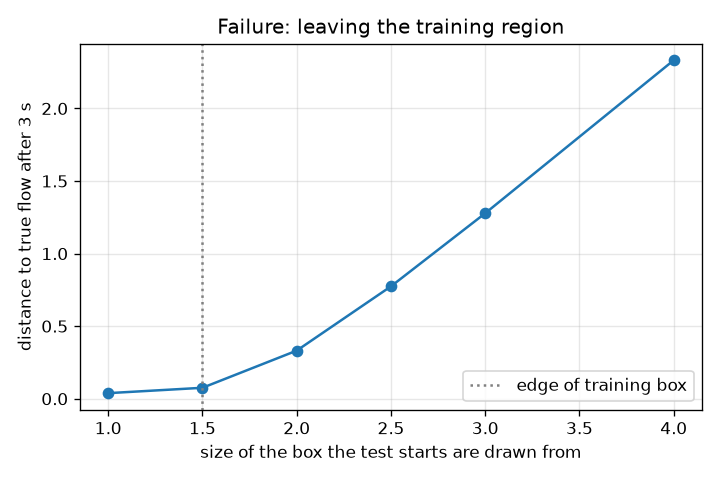
\includegraphics[width=0.85\linewidth]{figures/s03_extrapolation.png}\\\small Failure case: the error after 3 s against the size of the box the test starts are drawn from; the dotted line is the training box.\end{center}

\subsection*{E. Worked example}
A stiff system has x' = -1000 x. With RK4 and h = 0.01 s, what happens? What is the largest stable step, and what happens at h = 0.002 s?
\begin{enumerate}[nosep]
\item z = lambda h = -1000 * 0.01 = -10.
\item R(-10) = 1 - 10 + 50 - 166.67 + 416.67 = 291. Each step multiplies the state by 291, while the true solution decays: the numerical solution explodes.
\item The stability limit on the negative real axis is z = -2.785, so h must be at most 2.785 / 1000 = 0.0028 s (more exactly 0.002785 s).
\item At h = 0.002: z = -2 and R(-2) = 1 - 2 + 2 - 1.3333 + 0.6667 = 1/3. The state shrinks by a third each step: stable.
\end{enumerate}
\textbf{Answer.} At h = 0.01 the factor is 291 per step (blow-up); the largest stable step is about 0.0028 s; at h = 0.002 s the factor is 1/3 (stable).

\subsection*{F. Questions}
\begin{enumerate}[nosep]
\item \textbf{Conceptual.} Why does rollout training give better long predictions than one-step training when the data are noisy?
\item \textbf{Numerical.} For lambda = -500 per s, find the largest stable RK4 step. Does h = 0.01 s work? Give R(z) for h = 0.004 s and state the units.
\item \textbf{Graph and simulation interpretation.} In the error view, set the horizon to 8 and the noise to 0.0, 0.05 and 0.1. What happens to the error after 6 s, and why does the curve not grow without bound over time?
\item \textbf{Design and optimisation challenge.} Design: the sensor noise is 0.1 and you need an error below 0.1 after 6 s. You can record 6 or 18 runs with the same 25 samples each. Which would you choose, and what are the trade-offs?
\end{enumerate}

\section{Real-world mini-project}
\textbf{Learn a damped pendulum from noisy data and predict forward.} A lab records a damped pendulum with a noisy angle sensor: 8 runs of 31 samples, 0.1 s apart, starting at random angles and speeds between -2 and 2 (rad, rad/s), noise sigma = 0.03. The rule is theta' = omega and omega' = -4 sin(theta) - 0.3 omega, but pretend you do not know it. Use \texttt{pendulum\_model} from Session 3 (a 16-unit Neural ODE trained on 8-step rollouts) and predict 6 s ahead from 20 unseen starting states between -1.8 and 1.8. Compare with the small-angle model that replaces sin(theta) by theta.

\section{The path ahead}
\begin{enumerate}[nosep]
\item \textbf{Session 4: The adjoint method.} A gradient routine that integrates the adjoint equations backwards instead of storing the RK4 stages.
\item \textbf{Session 5: A limit cycle: Van der Pol.} A Neural ODE for the Van der Pol oscillator with a curriculum on the rollout length.
\item \textbf{Session 6: Stiff dynamics with an implicit solver.} Backward Euler or an adaptive solver inside the rollout.
\item \textbf{Session 7: Learning under heavy noise.} A training recipe that stays accurate at noise 0.1 with only 6 runs.
\item \textbf{Session 8: Hidden velocity: partial observation.} A model that sees only the position of the oscillator and learns the velocity as a hidden state.
\end{enumerate}

\section{Answers and hints}

\subsection*{Session 1}
\begin{enumerate}[nosep]
\item \textbf{Conceptual.} Hint: The first number is dx/dt, the speed. What is the speed at this state? Solution: The first number is dx/dt = v, and at this state v = 0: the mass is momentarily at rest at the end of its swing. It is the second number, dv/dt = -4, that says the velocity is about to change. The arrow tells how the state is changing now, not where the mass will be; position changes only after the velocity has changed.
\item \textbf{Numerical.} Hint: dx/dt = v and dv/dt = -k x - c v. New state = old state + 0.1 * arrow. Solution: Arrow = (2 m/s, -0.8 m/s\textasciicircum{}2). New state = (0, 2) + 0.1 * (2, -0.8) = (0.2 m, 1.92 m/s). Sanity check: in 0.1 s at about 2 m/s the mass moves about 0.2 m, and friction takes about 0.08 m/s off the speed. Both match.
\item \textbf{Graph and simulation interpretation.} Hint: Energy per unit mass is 0.5 (v\textasciicircum{}2 + k x\textasciicircum{}2). What does friction do to it? Solution: Friction removes energy, so each loop is smaller: with c = 0.4 the energy has fallen to below a fifth of its start after 6 s. With c = 0 nothing removes energy, so the path repeats the same loop forever (the energy stays 2.0 for the start (1, 0)). With friction the path ends at the centre (0, 0): the mass at rest at the rest point.
\item \textbf{Design and optimisation challenge.} Hint: Use arrow\_error(dt) in the lesson: the largest relative gap between estimated and true arrows. Solution: At dt = 0.25 s the gap is between 1 and 3 percent, so it fails the 1 percent requirement; at dt = 0.1 s the gap is below 1 percent, so it passes. Trade-off: a faster sensor gives better arrows, but with a real sensor noise is multiplied by 1/dt, so you cannot make dt arbitrarily small (Session 2 shows this).
\end{enumerate}

\subsection*{Session 2}
\begin{enumerate}[nosep]
\item \textbf{Conceptual.} Hint: Where does the noise end up when you form derivatives and when you use noisy positions as inputs? Solution: Two effects do not average away. Derivative estimates divide noise by 2 dt, so each derivative is very noisy. And the noisy positions are also the inputs of the fit, which biases a least-squares line (it pulls the fitted rule towards zero). Averaging more runs reduces the random part but not this bias, so the error flattens at a floor set by the noise level. Only less noise (a better sensor) or a better method lowers it.
\item \textbf{Numerical.} Hint: Error scales like h\textasciicircum{}p: dividing h by 4 divides the error by 4\textasciicircum{}p. Solution: Euler: 0.575 / 4 = 0.144, measured 0.128; the guess is close but not exact because the step is still coarse. RK4: 4.3e-5 / 4\textasciicircum{}4 = 4.3e-5 / 256 = 1.7e-7. Units: distance in state space (m and m/s mixed, as one number). Sanity check: RK4 needs 4 arrow evaluations per step but a 4 times smaller step is not needed, so it is far cheaper for the same accuracy.
\item \textbf{Graph and simulation interpretation.} Hint: Slope on log-log axes is the exponent of h. At some point other errors take over. Solution: The slope of the straight line is the exponent p in error = C h\textasciicircum{}p: a slope of 2 would mean that halving h divides the error by 4. For extremely small h, rounding errors of the computer (about 1e-16 relative) dominate and the curve flattens, so decreasing h further no longer helps.
\item \textbf{Design and optimisation challenge.} Hint: Use mean\_fit\_error(K, sigma) from the lesson; remember that extra runs cost time. Solution: Noise 0.01 passes with a single run (below 0.1). Noise 0.05 fails with 1 run (above 0.1), just passes on average with 3 runs (between 0.08 and 0.1, so with little margin) and passes safely with 10 runs. Noise 0.2 fails for every K (above 0.3 even with 30 runs). Choice: the 0.05 sensor with 10 runs is a safe passing design; a sensor with noise 0.2 cannot be rescued by more data. Trade-off: a 0.01 sensor costs more but needs one run.
\end{enumerate}

\subsection*{Session 3}
\begin{enumerate}[nosep]
\item \textbf{Conceptual.} Hint: In one-step training what is the target of each step, and what does the model see about the later steps? Solution: In one-step training each target is a single noisy next point close to the input, so the noise in it is as large as the change the model must learn, and noise in the input is treated as truth. Errors are never compounded during training, so small mistakes in the arrows that pile up over many steps are not penalised. In rollout training the loss is measured after 8 steps, where the signal (the true motion) is larger relative to the noise and the compounding of errors is part of the loss. The model is therefore pushed to be right over the horizon we care about. In the lesson, one-step training is more than twice as bad after 6 s.
\item \textbf{Numerical.} Hint: The stability limit is z = lambda h = -2.785. Solution: h\_max = 2.785 / 500 = 0.00557 s. For h = 0.01: z = -5, which is beyond the limit, so it is unstable (\textbar{}R(-5)\textbar{} is above 1). For h = 0.004: z = -2, R = 1/3, stable. R has no unit; h is in seconds. Sanity check: a faster process (larger \textbar{}lambda\textbar{}) needs a smaller step.
\item \textbf{Graph and simulation interpretation.} Hint: Compare the blue curve at 6 s for the three noise levels. What does the true system do at long times? Solution: The error rises with noise: it is several times larger at noise 0.1 than with no noise. It does not grow without bound because the true system is damped: both the true and the learned flow decay towards rest, so the distance between them is bounded by their own sizes. (For an unstable or chaotic system the error would grow.)
\item \textbf{Design and optimisation challenge.} Hint: Use design\_error(n\_traj, sigma) in the lesson (worst error over two random data sets). Solution: With 6 runs the worst error over two data sets is above 0.1 so it fails; with 18 runs the worst error is below 0.1, so it passes. So choose 18 runs (3 times the data and about 3 times the training time), or, if recording is costly, buy a better sensor (noise 0.05 with 6 runs also passes). Trade-offs: more data costs recording time and training time, and it does not remove the risk when the noise is much larger.
\end{enumerate}

\section{How to join}
Read \texttt{CONTRIBUTING.md} in the repository, then pick an issue labelled \texttt{good first issue}. Repository: \url{https://github.com/KrunalPanchal1995/pan-iit-oss/tree/main/openneuralode}

\end{document}
